\documentclass[11pt,a4paper]{article}

% ---------- Pacchetti ----------
\usepackage[a4paper,margin=2.7cm,headheight=28pt]{geometry}
\usepackage[utf8]{inputenc}
\usepackage[T1]{fontenc}
\usepackage{graphicx}
\usepackage{xcolor}
\usepackage{booktabs}
\usepackage{longtable}
\usepackage{array}
\usepackage{fancyhdr}
\usepackage{hyperref}
\usepackage{enumitem}
\usepackage{titlesec}
\usepackage{tabularx}
\usepackage{colortbl}
\usepackage{needspace}
\usepackage[most]{tcolorbox}
\usepackage{seqsplit}

% ---------- Colori SkyNet ----------
\definecolor{skyblue}{HTML}{4DA6F0}
\definecolor{skyblueLight}{HTML}{AEDBFA}
\definecolor{skydark}{HTML}{1B1B1B}
\definecolor{noteBg}{HTML}{EAF4FF}
\definecolor{warnBg}{HTML}{FFF3E0}

% ---------- Colori semantici di stato (coerenti con il Design System) ----------
\definecolor{stAttesa}{HTML}{9E9E9E}
\definecolor{stElaborazione}{HTML}{3B82F6}
\definecolor{stCompletato}{HTML}{22A55A}
\definecolor{stFallito}{HTML}{DC2626}
\definecolor{stAnnullato}{HTML}{6B7280}

% ---------- Titoli sezione ----------
\titleformat{\section}{\Large\bfseries\color{skydark}}{\thesection}{0.6em}{}
\titleformat{\subsection}{\large\bfseries\color{skydark}}{\thesubsection}{0.6em}{}
\titleformat{\subsubsection}{\normalsize\bfseries\color{skydark}}{\thesubsubsection}{0.6em}{}

% ---------- Intestazione/piede pagina ----------
\pagestyle{fancy}
\fancyhf{}
\renewcommand{\headrulewidth}{0.4pt}
\renewcommand{\footrulewidth}{0.4pt}
\fancyhead[L]{\small\leftmark}
\fancyhead[R]{
\includegraphics[height=11pt]{figures/logo_skynet_dark.png}}
\fancyfoot[L]{\small Manuale Utente — Code Guardian}
\fancyfoot[R]{\small\thepage}
\renewcommand{\sectionmark}[1]{\markboth{#1}{}}

% ---------- Link ----------
\hypersetup{
  colorlinks=true,
  linkcolor=black,
  citecolor=black,
  urlcolor=skyblue!70!black,
  pdftitle={Manuale Utente - Code Guardian},
  pdfauthor={Gruppo SkyNet}
}

% ---------- Comandi ausiliari ----------
\newcommand{\route}[1]{\texttt{#1}}
\newcommand{\code}[1]{\texttt{#1}}
\newcommand{\ecode}[1]{\texttt{\seqsplit{#1}}}

\newtcolorbox{nota}{
  enhanced, breakable, colback=noteBg, colframe=skyblue!60!black,
  boxrule=0.5pt, arc=2pt, left=8pt, right=8pt, top=5pt, bottom=5pt,
  before skip=8pt, after skip=8pt,
  title=Nota, fonttitle=\bfseries, coltitle=black,
  attach title to upper={\bfseries\ --- }, colbacktitle=noteBg,
  boxsep=0pt, toptitle=0pt, bottomtitle=0pt
}

\newtcolorbox{avviso}{
  enhanced, breakable, colback=warnBg, colframe=orange!70!black,
  boxrule=0.5pt, arc=2pt, left=8pt, right=8pt, top=5pt, bottom=5pt,
  before skip=8pt, after skip=8pt,
  title=Attenzione, fonttitle=\bfseries, coltitle=black,
  attach title to upper={\bfseries\ --- }, colbacktitle=warnBg,
  boxsep=0pt, toptitle=0pt, bottomtitle=0pt
}

\setlist[itemize]{leftmargin=1.4em}
\setlist[enumerate]{leftmargin=1.6em}

\begin{document}

% ============================================================
% COPERTINA
% ============================================================
\begin{titlepage}
\thispagestyle{empty}
\begin{center}
\vspace*{2.5cm}

\includegraphics[width=0.5\textwidth]{figures/logo_skynet_dark.png}

\vspace{1.2cm}
{\large Gruppo SkyNet}\\
{\small \href{mailto:skynetunigroup@gmail.com}{skynetunigroup@gmail.com}}

\vspace{2.2cm}
{\Huge\bfseries Manuale Utente}

\vspace{0.4cm}
{\Large Code Guardian}

\vspace{2.5cm}

\renewcommand{\arraystretch}{1.35}
\begin{tabular}{|p{3.4cm}|p{8.4cm}|}
\hline
\textbf{Versione} & 1.0.0 \\
\hline
\textbf{Uso} & \textit{Utenti finali di Code Guardian} \\
\hline
\textbf{Redattori} & \textit{Samuele Bertin} \\
\hline
\textbf{Verifica} & \textit{Dario Pirrone, Andrea Fistarol} \\
\hline
\textbf{Approvazione} & \textit{Dario Pirrone, Marco Barbiero} \\
\hline
\end{tabular}

\end{center}
\end{titlepage}

% ============================================================
% VERSIONI DEL DOCUMENTO
% ============================================================
\newpage
\thispagestyle{plain}
\section*{Versioni del documento}
\renewcommand{\arraystretch}{1.3}
\begin{tabularx}{\textwidth}{|c|c|X|c|c|}
\hline
\textbf{Versione} & \textbf{Data} & \textbf{Descrizione} & \textbf{Autore} & \textbf{Verificatore}\\
\hline

1.0.0 & 2026/09/24 & Approvazione per la revisione PB & Marco Barbiero & - \\ \hline
0.5.0 & 2026/09/20 & Allineamento del Manuale alle modalità operative effettive. Controllo ortografico e di presentazione del documento. & Andrea Fistarol & Edoardo Granziero \\ \hline
0.4.0 & 2026/09/06 & Risoluzione dei problemi ed errori, Glossario. & Samuele Bertin & Dario Pirrone \\ \hline
0.3.0 & 2026/09/05 & Funzionalità AI. & Samuele Bertin & Dario Pirrone \\ \hline
0.2.0 & 2026/09/04 & Installazione e Avvio, Guida all'interfaccia. & Samuele Bertin & Dario Pirrone \\ \hline
0.1.0 & 2026/09/03 & Prima stesura del Manuale Utente: Introduzione. & Samuele Bertin & Dario Pirrone \\
\hline
\end{tabularx}

\vspace{1cm}

% ============================================================
% INDICE
% ============================================================
\newpage
\tableofcontents

% ============================================================
\newpage
\section{Introduzione}

\subsection{Cos'è Code Guardian}

Code Guardian è un'applicazione web che automatizza l'audit, la manutenzione e la
documentazione dei repository software ospitati su GitHub. Una volta collegato il proprio
repository, l'utente può richiedere a tre agenti intelligenti, basati su modelli linguistici
di grandi dimensioni (LLM), di analizzare il codice e produrre in autonomia:

\begin{itemize}
  \item documentazione tecnica aggiornata (README, commenti inline, documentazione degli
        Endpoint);
  \item una scansione delle vulnerabilità di sicurezza più comuni;
  \item un changelog leggibile a partire dalle User Story completate in uno Sprint.
\end{itemize}

Ogni analisi produce un \textbf{report} strutturato, consultabile nell'interfaccia e
scaricabile in formato PDF. Quando un agente propone una modifica ai file del progetto
(ad esempio un nuovo README), Code Guardian apre automaticamente una \textbf{Pull Request}
su GitHub: nessuna modifica viene mai scritta direttamente sul repository senza che
sia l'utente, tramite il normale flusso di revisione di GitHub, ad approvarla.

\subsection{A chi è rivolto questo manuale}

Questo manuale è rivolto a chiunque utilizzi Code Guardian come utente finale: sviluppatori,
security auditor/team lead e project manager. Non tratta argomenti di infrastruttura o di
amministrazione del sistema (hosting, configurazione dei server, gestione del database), che
restano di competenza del team che opera e mantiene l'applicazione.

\subsection{I tre agenti in breve}

\begin{itemize}
  \item \textbf{Agente Docs} --- genera e aggiorna la documentazione del progetto: il file
        \code{README.md}, i commenti di codice (JSDoc/docstring) e un documento
        \code{API.md} con l'elenco degli Endpoint. Propone sempre le modifiche tramite
        Pull Request.
  \item \textbf{Agente Security} --- analizza il codice alla ricerca di vulnerabilità
        riconducibili alla OWASP Top 10 e verifica la conformità del progetto alle regole
        definite nel file \code{POLICY.md}. Segnala i problemi riscontrati ma non modifica
        mai il codice: la correzione resta un'attività umana.
  \item \textbf{Agente Changelog} --- legge le User Story completate in uno Sprint da GitHub
        Issues e genera un changelog tecnico, orientato allo sviluppo, e, su richiesta, un
        changelog di business più leggibile per un pubblico non tecnico.
\end{itemize}

\subsection{Ruoli operativi}

Ogni utente sceglie un ruolo in fase di registrazione, che resta fisso per tutta la vita
dell'account e determina quali operazioni sono disponibili nella schermata di avvio. La
Tabella~\ref{tab:ruoli} riassume la mappatura.

\begin{table}[h]
\centering
\renewcommand{\arraystretch}{1.3}
\begin{tabularx}{\textwidth}{|>{\raggedright\arraybackslash}p{3.1cm}|X|>{\centering\arraybackslash}p{2.0cm}|}
\hline
\textbf{Ruolo} & \textbf{Operazioni disponibili} & \textbf{Agente} \\
\hline
Sviluppatore & Generazione/aggiornamento README, documentazione inline (JSDoc), documentazione API & Docs \\
\hline
Security Auditor / Team Lead & Scansione vulnerabilità OWASP Top 10, verifica conformità Policy-as-code & Security \\
\hline
Project Manager & Changelog di business & Changelog \\
\hline
Project Manager e Sviluppatore & Changelog tecnico & Changelog \\
\hline
\end{tabularx}
\caption{Operazioni disponibili per ciascun ruolo operativo.}
\label{tab:ruoli}
\end{table}

Tutti i ruoli condividono inoltre le funzionalità trasversali dell'applicazione: selezione
del repository, configurazione delle credenziali, monitoraggio delle operazioni in corso e
consultazione dello storico dei report. Le operazioni non permesse al proprio ruolo non
vengono mostrate come disabilitate: semplicemente non compaiono nell'elenco.

% ============================================================
\newpage
\section{Installazione e Avvio}

Code Guardian è un'applicazione interamente web-based: non richiede alcuna installazione
sul proprio computer. È sufficiente un browser aggiornato per accedervi.

\subsection{Requisiti}

\begin{itemize}
  \item Un browser desktop recente e aggiornato: Google Chrome, Mozilla Firefox oppure
        Microsoft Edge (versione 145 o superiore).
  \item Un account GitHub con un Personal Access Token (PAT) con permesso \code{repo},
        per collegare i propri repository (si veda la sezione~\ref{sec:credenziali}).
  \item L'indirizzo (URL) dell'ambiente Code Guardian fornito dal proprio team o
        amministratore.
\end{itemize}

\begin{avviso}
Il token di sessione dell'utente non viene mai salvato nella memoria persistente del browser.
Questo significa che, ricaricando completamente la pagina, è necessario effettuare di nuovo
l'accesso: si tratta di una scelta di sicurezza, non di un malfunzionamento.
\end{avviso}

\subsection{Creazione dell'account}

Al primo utilizzo occorre creare un account dalla pagina \route{/register}:

\begin{enumerate}
  \item inserire nome e cognome;
  \item inserire un indirizzo email valido (verrà validato mentre si compila il campo);
  \item scegliere una password di almeno 8 caratteri, con almeno una lettera e una cifra;
  \item selezionare il proprio ruolo operativo iniziale: Sviluppatore, Security Auditor /
        Team Lead oppure Project Manager (si veda la sezione~\ref{sec:ruoli-dettaglio} per
        le differenze);
  \item confermare con il pulsante \textbf{Crea account}.
\end{enumerate}

Se l'indirizzo email è già registrato, compare un messaggio non bloccante con un collegamento
diretto alla pagina di accesso. La registrazione non effettua l'accesso automatico: una volta
creato l'account occorre accedere separatamente da \route{/login}.

\newpage
\begin{nota}
Il ruolo scelto in fase di registrazione resta fisso per tutta la vita dell'account: non
esiste, in questa versione dell'applicazione, una funzione per cambiarlo in un secondo
momento.
\end{nota}

\subsection{Accesso (Login)}

Dalla pagina \route{/login}, inserire l'indirizzo email e la password scelti in fase di
registrazione e confermare con \textbf{Accedi}. In caso di credenziali non corrette, viene
mostrato un unico messaggio generico (per non rivelare se l'errore riguarda l'email o la
password). La sessione resta attiva per 8 ore o fino al ricaricamento completo della pagina.

Dopo l'accesso, l'applicazione reindirizza automaticamente l'utente:

\begin{itemize}
  \item alla pagina \route{/credentials}, se non è ancora stato configurato alcun servizio
        esterno;
  \item alla pagina \route{/select}, se una credenziale GitHub è già configurata e valida.
\end{itemize}

\subsection{Configurazione dei servizi esterni (GitHub)}
\label{sec:credenziali}

Nessuna operazione degli agenti è raggiungibile senza aver prima collegato un account
GitHub. Sulla pagina \route{/credentials}:

\begin{enumerate}
  \item inserire il proprio Personal Access Token GitHub con permesso \code{repo} nel
        campo dedicato;
  \item confermare con \textbf{Connetti}: il sistema esegue prima un controllo di formato,
        poi una chiamata di verifica a GitHub; la credenziale viene salvata solo se
        entrambi i controlli hanno esito positivo;
  \item una volta connesso, il servizio mostra l'etichetta \textbf{Connesso} con la data
        dell'ultima verifica riuscita.
\end{enumerate}

Lo stesso token copre sia la lettura del codice sia l'accesso alle GitHub Issues, usate
dall'Agente Changelog come sistema di gestione dei task: non è quindi necessario configurare
due credenziali separate.

\begin{nota}
In qualunque momento è possibile premere \textbf{Verifica di nuovo} per controllare che il
token sia ancora valido, oppure \textbf{Rimuovi} per revocarlo localmente (l'operazione non
revoca il token anche su GitHub: per farlo occorre agire direttamente sul proprio account
GitHub).
\end{nota}

\subsection{Primo utilizzo: selezione del contesto operativo}

Completata la configurazione delle credenziali, si accede alla pagina \route{/select} per
definire su cosa dovranno lavorare gli agenti (si veda la sezione~\ref{sec:select} per il
dettaglio dei campi). Una volta salvato, il contesto resta valido per tutte le operazioni
avviate nella stessa sessione di lavoro; agli accessi successivi, un utente già configurato
salta direttamente alla pagina \route{/run} o a \route{/select} se desidera cambiare
repository.

% ============================================================
\newpage
\section{Guida all'interfaccia}
\label{sec:ruoli-dettaglio}

\subsection{Mappa di navigazione}

La Figura~\ref{fig:navmap} riassume le pagine principali dell'applicazione e i percorsi che
un utente segue normalmente per andare dall'accesso all'avvio di un'operazione e alla
consultazione del relativo report.

\begin{figure}[h]
\centering
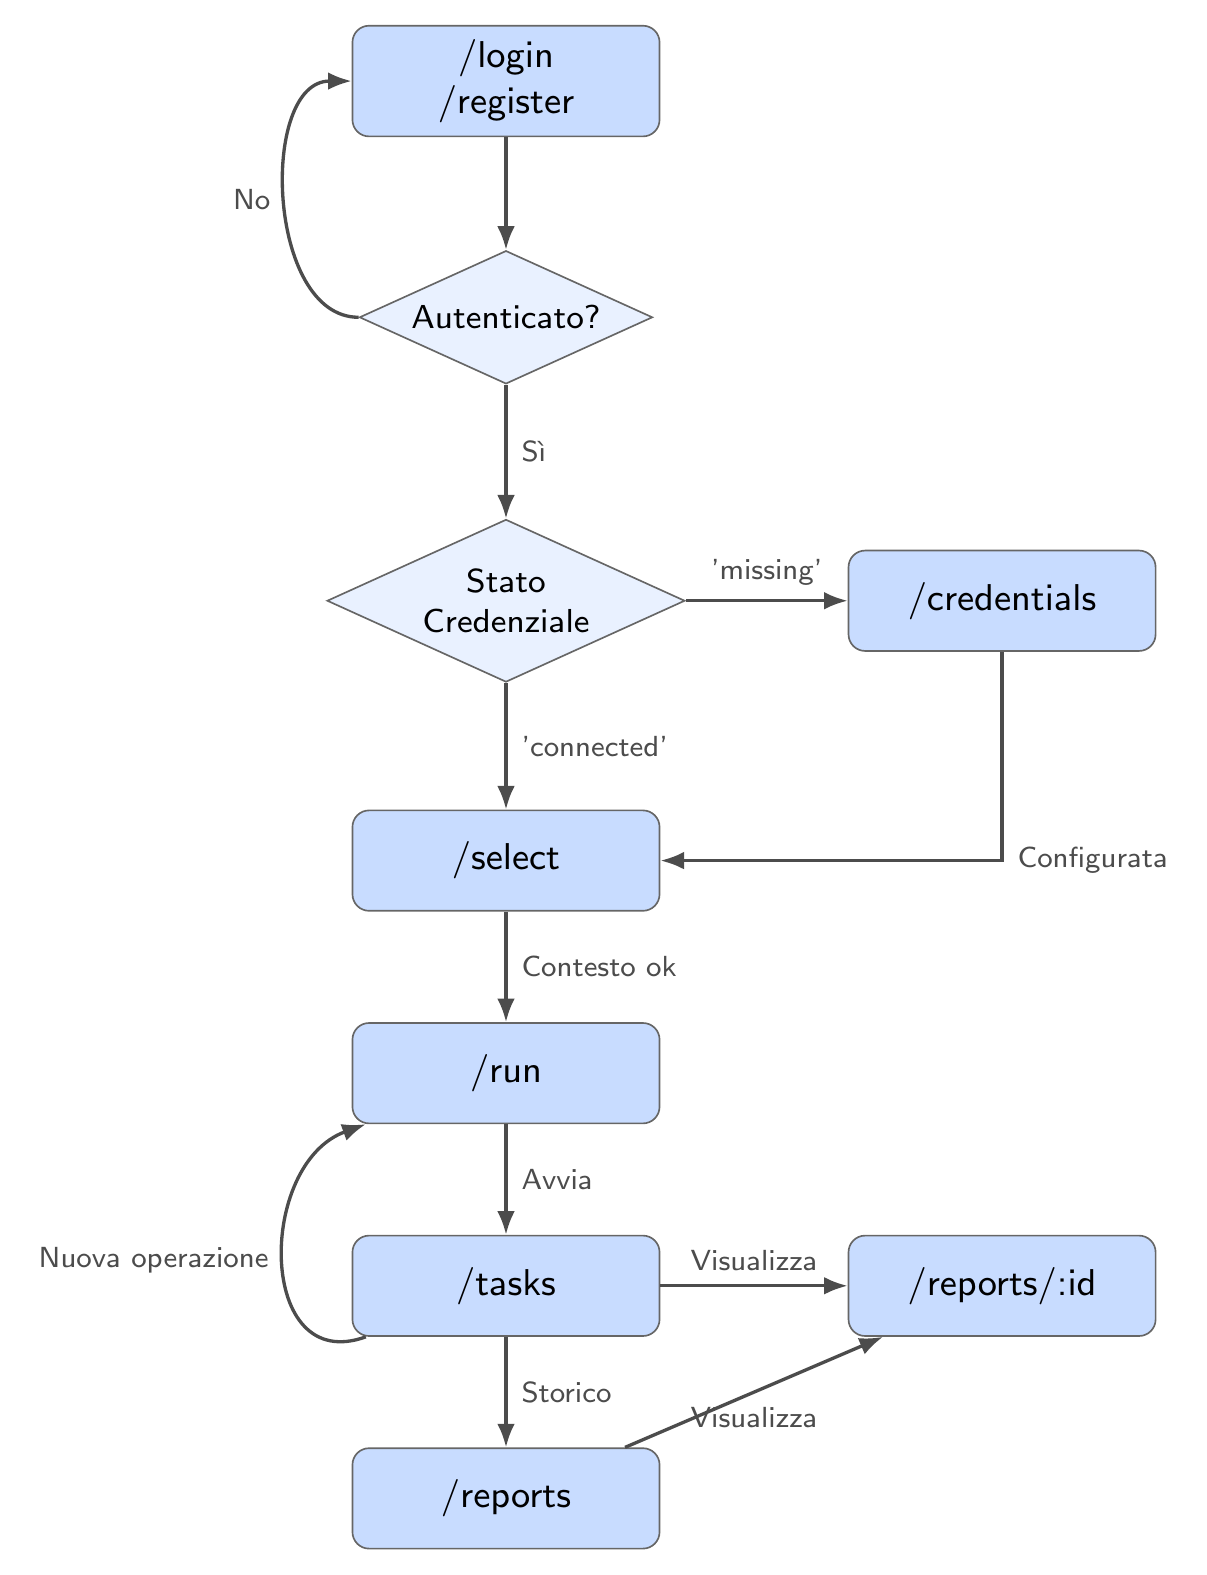
\includegraphics[width=0.62\textwidth]{figures/mappa_navigazione.png}
\caption{Mappa di navigazione principale dell'applicazione.}
\label{fig:navmap}
\end{figure}

\subsection{Intestazione applicativa}

Un'intestazione persistente compare su tutte le pagine successive all'accesso e mostra:

\begin{itemize}
  \item il nome dell'utente autenticato;
  \item un'etichetta con il ruolo operativo assegnato;
  \item un banner di avviso, quando la credenziale GitHub non è più valida (si veda la
        sezione~\ref{sec:credenziale-invalida}), con un collegamento diretto a
        \route{/credentials};
  \item il comando \textbf{Esci}, che chiude la sessione corrente.
\end{itemize}

\subsection{Servizi connessi --- \texttt{/credentials}}

Elenca i servizi esterni collegabili (nell'attuale versione, solo GitHub) con il relativo
stato: non configurato, connesso oppure non più valido. È la pagina descritta in
dettaglio nella sezione~\ref{sec:credenziali}.

\subsection{Selezione del contesto --- \texttt{/select}}
\label{sec:select}

Questa pagina definisce \emph{su cosa} lavoreranno gli agenti. È divisa in due aree.

\paragraph{Repository e riferimento.}
\begin{itemize}
  \item \textbf{URL del repository} --- l'indirizzo del repository GitHub da analizzare.
  \item \textbf{Branch} --- il nome del ramo di riferimento; una volta validato l'URL,
        il campo propone un autocompletamento con i branch disponibili.
  \item \textbf{Hash del commit} (opzionale) --- per ancorare l'analisi a un commit
        specifico anziché all'ultimo dello stato attuale del branch.
\end{itemize}

\paragraph{Ambito di analisi.}
Una volta validato il repository, si sceglie \emph{quanto} del repository analizzare:

\begin{itemize}
  \item \textbf{Intero repository} --- comando rapido che seleziona tutto il contenuto;
  \item \textbf{File o cartelle specifici} --- si deve poi inserire nella casella di testo sottostante l'indirizzo o gli indirizzi dei file o delle cartelle da esaminare.
\end{itemize}

\begin{nota}
Solo i file scritti in un linguaggio supportato (TypeScript, JavaScript o Python) vengono
effettivamente considerati dagli agenti. Se il repository contiene altri linguaggi, compare
un avviso non bloccante: l'analisi prosegue comunque sui file supportati.
\end{nota}

\subsection{Avvio operazioni --- \texttt{/run}}

Mostra l'elenco delle operazioni disponibili per il proprio ruolo (si veda la
Tabella~\ref{tab:ruoli}), ciascuna con nome e breve descrizione. È
possibile selezionare più operazioni contemporaneamente e avviarle in un'unica conferma con
il pulsante \textbf{Avvia}: ciascuna diventerà un elemento indipendente nella Dashboard. Il
pulsante resta disabilitato finché non è selezionata almeno un'operazione.

\begin{nota}
L'operazione \emph{Changelog di business} non richiede di selezionare anche il
\emph{Changelog tecnico}: la generazione del changelog tecnico è inclusa automaticamente
come primo passo dell'operazione di business (si veda la sezione~\ref{sec:agente-changelog}).
\end{nota}

\subsection{Dashboard --- \texttt{/tasks}}
\label{sec:dashboard}

La Dashboard elenca le operazioni avviate nella sessione corrente e ne mostra l'avanzamento
in tempo reale, senza necessità di ricaricare la pagina. Per ciascuna operazione sono
visibili il nome, un indicatore di stato con barra di avanzamento, e i comandi disponibili.

\begin{figure}[h]
\centering
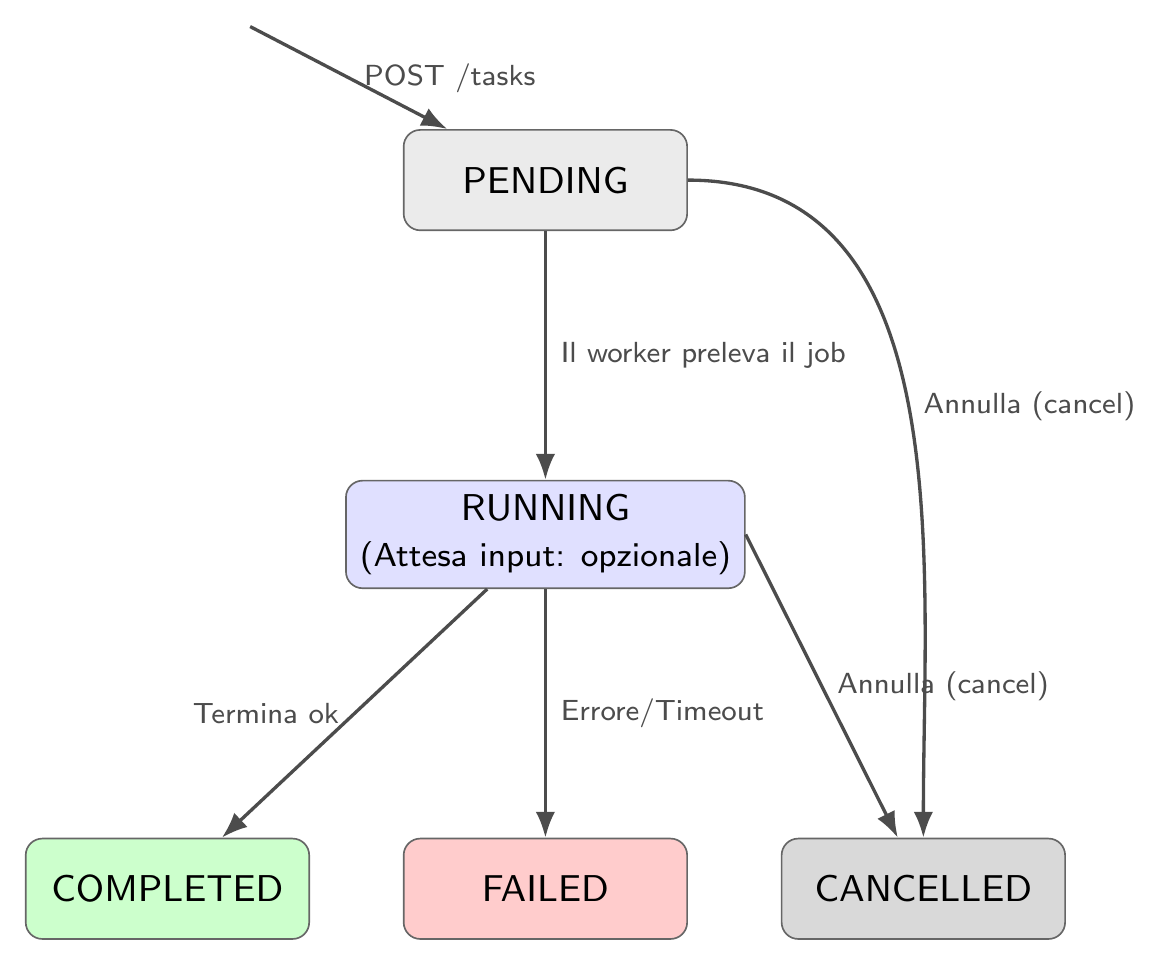
\includegraphics[width=0.62\textwidth]{figures/ciclo_vita_task.png}
\caption{Ciclo di vita di un'operazione (Task) mostrata in Dashboard.}
\label{fig:lifecycle}
\end{figure}

Ogni operazione attraversa gli stati mostrati in Figura~\ref{fig:lifecycle}:

\begin{itemize}
  \item \textbf{In attesa} --- l'operazione è stata accodata mentre attende una risorsa
        disponibile;
  \item \textbf{In elaborazione} --- l'agente sta analizzando il contenuto selezionato
        (è in questo stato che, per l'Agente Changelog, possono comparire richieste di
        input, si veda la sezione~\ref{sec:agente-changelog});
  \item \textbf{Completato} --- il report è pronto e consultabile;
  \item \textbf{Fallito} --- l'operazione si è interrotta per un errore (si veda la
        sezione~\ref{sec:errori});
  \item \textbf{Annullato} --- l'operazione è stata interrotta dall'utente con il comando
        \textbf{Annulla}, disponibile finché l'operazione è in attesa o in elaborazione.
\end{itemize}

\begin{nota}
Le operazioni avviate insieme vengono eseguite una alla volta, non in parallelo: se si
avviano più operazioni contemporaneamente, alcune resteranno nello stato \textbf{In
attesa} finché l'agente non si libera dall'elaborazione precedente. Il fallimento di
un'operazione, in ogni caso, non blocca né invalida quelle in coda dopo di essa.
\end{nota}

Il comando \textbf{Visualizza report} è disponibile per le operazioni completate o fallite.
Il fallimento di un'operazione è sempre isolato al singolo elemento della lista: le altre
operazioni del batch proseguono senza interruzioni.

\subsection{Storico e dettaglio dei report --- \texttt{/reports}, \texttt{/reports/:id}}

La pagina \route{/reports} elenca tutti i report generati dall'utente, con identificativo,
titolo descrittivo (nome dell'operazione, repository e branch analizzati) e data/ora di
generazione. Selezionando un elemento si apre la pagina di dettaglio \route{/reports/:id},
raggiungibile anche direttamente dalla Dashboard subito dopo il completamento di
un'operazione.

La pagina di dettaglio mostra, nell'intestazione, repository, riferimento, ambito analizzato
e tempo di esecuzione; nel corpo, il contenuto del report nel formato più adatto al tipo di
operazione (testo Markdown, elenco di riscontri, collegamento alla Pull Request --- si veda
la sezione~\ref{sec:funzionalita-ai}). Da qui è sempre disponibile il pulsante
\textbf{Esporta PDF}.

\subsection{Convenzioni visive}

\begin{itemize}
  \item \textbf{Colori di stato} --- ogni indicatore di stato (Attesa, Elaborazione,
        Completato, Fallito, Annullato) ha un colore coerente in tutta l'applicazione,
        sempre accompagnato da un'etichetta testuale.
  \item \textbf{Colori di gravità} --- i riscontri dell'Agente Security e gli avvisi di
        complessità dell'Agente Docs usano gli stessi cinque livelli: Critica, Alta,
        Media, Bassa, Informativa.
  \item \textbf{Blocchi di codice} --- gli snippet correttivi e i riferimenti a percorsi di
        file/righe sono mostrati con un font a spaziatura fissa, distinto dal testo
        dell'interfaccia.
  \item \textbf{Stati delle richieste} --- ogni azione che comporta una chiamata di rete
        mostra un indicatore di caricamento durante l'attesa e disabilita il comando che
        l'ha originata, per evitare invii duplicati.
\end{itemize}

% ============================================================
\newpage
\section{Funzionalità AI}
\label{sec:funzionalita-ai}

\subsection{Come funzionano gli agenti, in generale}

Ogni agente segue lo stesso schema di funzionamento:

\begin{enumerate}
  \item legge il codice (e, per il Changelog, le GitHub Issues) esclusivamente
        \emph{in lettura}, tramite l'accesso sicuro predisposto dall'applicazione --- gli
        agenti non ricevono mai direttamente il token GitHub dell'utente;
  \item elabora il contenuto con un modello linguistico (LLM), seguendo un modello di
        prompt specifico per l'operazione richiesta;
  \item restituisce un \textbf{report} strutturato, che l'applicazione mostra
        nell'interfaccia e rende disponibile per l'esportazione in PDF.
\end{enumerate}

\begin{nota}
Nessun agente scrive mai direttamente sul repository. Quando un'operazione prevede una
modifica ai file (l'Agente Docs), l'agente produce soltanto una \textbf{proposta} (un diff);
è l'applicazione stessa, non l'agente, ad aprire in automatico la Pull Request corrispondente
al termine dell'elaborazione.
\end{nota}

\subsection{Agente Docs}

Copre tre operazioni, tutte riservate al ruolo Sviluppatore e tutte concluse con l'apertura
automatica di una Pull Request:

\begin{itemize}
  \item \textbf{Generazione/aggiornamento README} --- produce o aggiorna il file
        \code{README.md} del progetto;
  \item \textbf{Documentazione inline} --- analizza il codice sorgente e propone commenti
        nella convenzione corretta (JSDoc per TypeScript/JavaScript, docstring per Python),
        sia per le unità di codice prive di documentazione sia per quelle la cui
        documentazione esistente non è più coerente con il codice;
  \item \textbf{Documentazione API} --- estrae le informazioni sugli Endpoint del progetto
        e genera un documento \code{API.md}.
\end{itemize}

Il report mostra come elemento principale il collegamento alla Pull Request aperta su
GitHub: la revisione e l'eventuale approvazione della modifica proposta avvengono
interamente su GitHub, con i normali strumenti di revisione (Code Guardian non prevede un
passaggio di approvazione interno). Per la documentazione inline e API, se una porzione di
codice è troppo complessa per essere documentata in modo affidabile, il report include un
avviso dedicato (a gravità informativa) invece di forzare un commento potenzialmente
scorretto.

\subsection{Agente Security}

Copre due operazioni, riservate al ruolo Security Auditor / Team Lead:

\begin{itemize}
  \item \textbf{Scansione vulnerabilità OWASP Top 10} --- analizza il codice alla ricerca
        di pattern riconducibili alle vulnerabilità più comuni (ad esempio SQL injection,
        cross-site scripting, segreti in chiaro, crittografia insicura, controllo accessi
        incompleto);
  \item \textbf{Verifica conformità Policy-as-code} --- confronta il progetto con le
        regole di sviluppo sicuro definite nel file \code{POLICY.md} presente nel
        repository.
\end{itemize}

Il report elenca i riscontri come lista filtrabile per gravità; per ciascun riscontro sono
indicati categoria, gravità, file e riga (quando disponibili) e un suggerimento di
correzione, sotto forma di uno snippet di codice quando il problema è sufficientemente
localizzato, oppure di una descrizione testuale in caso contrario.

\begin{avviso}
L'Agente Security individua e documenta i problemi, ma non li corregge né apre alcuna
Pull Request: la verifica e la correzione restano un'attività umana, a cura del Security
Auditor.
\end{avviso}

\subsection{Agente Changelog}
\label{sec:agente-changelog}

Copre due operazioni: il \textbf{Changelog tecnico} (Project Manager e Sviluppatore) e il
\textbf{Changelog di business} (solo Project Manager). È l'agente con il flusso più
interattivo, perché richiede alcune informazioni e conferme direttamente durante
l'elaborazione, senza che l'operazione venga interrotta.

\begin{figure}[h]
\centering
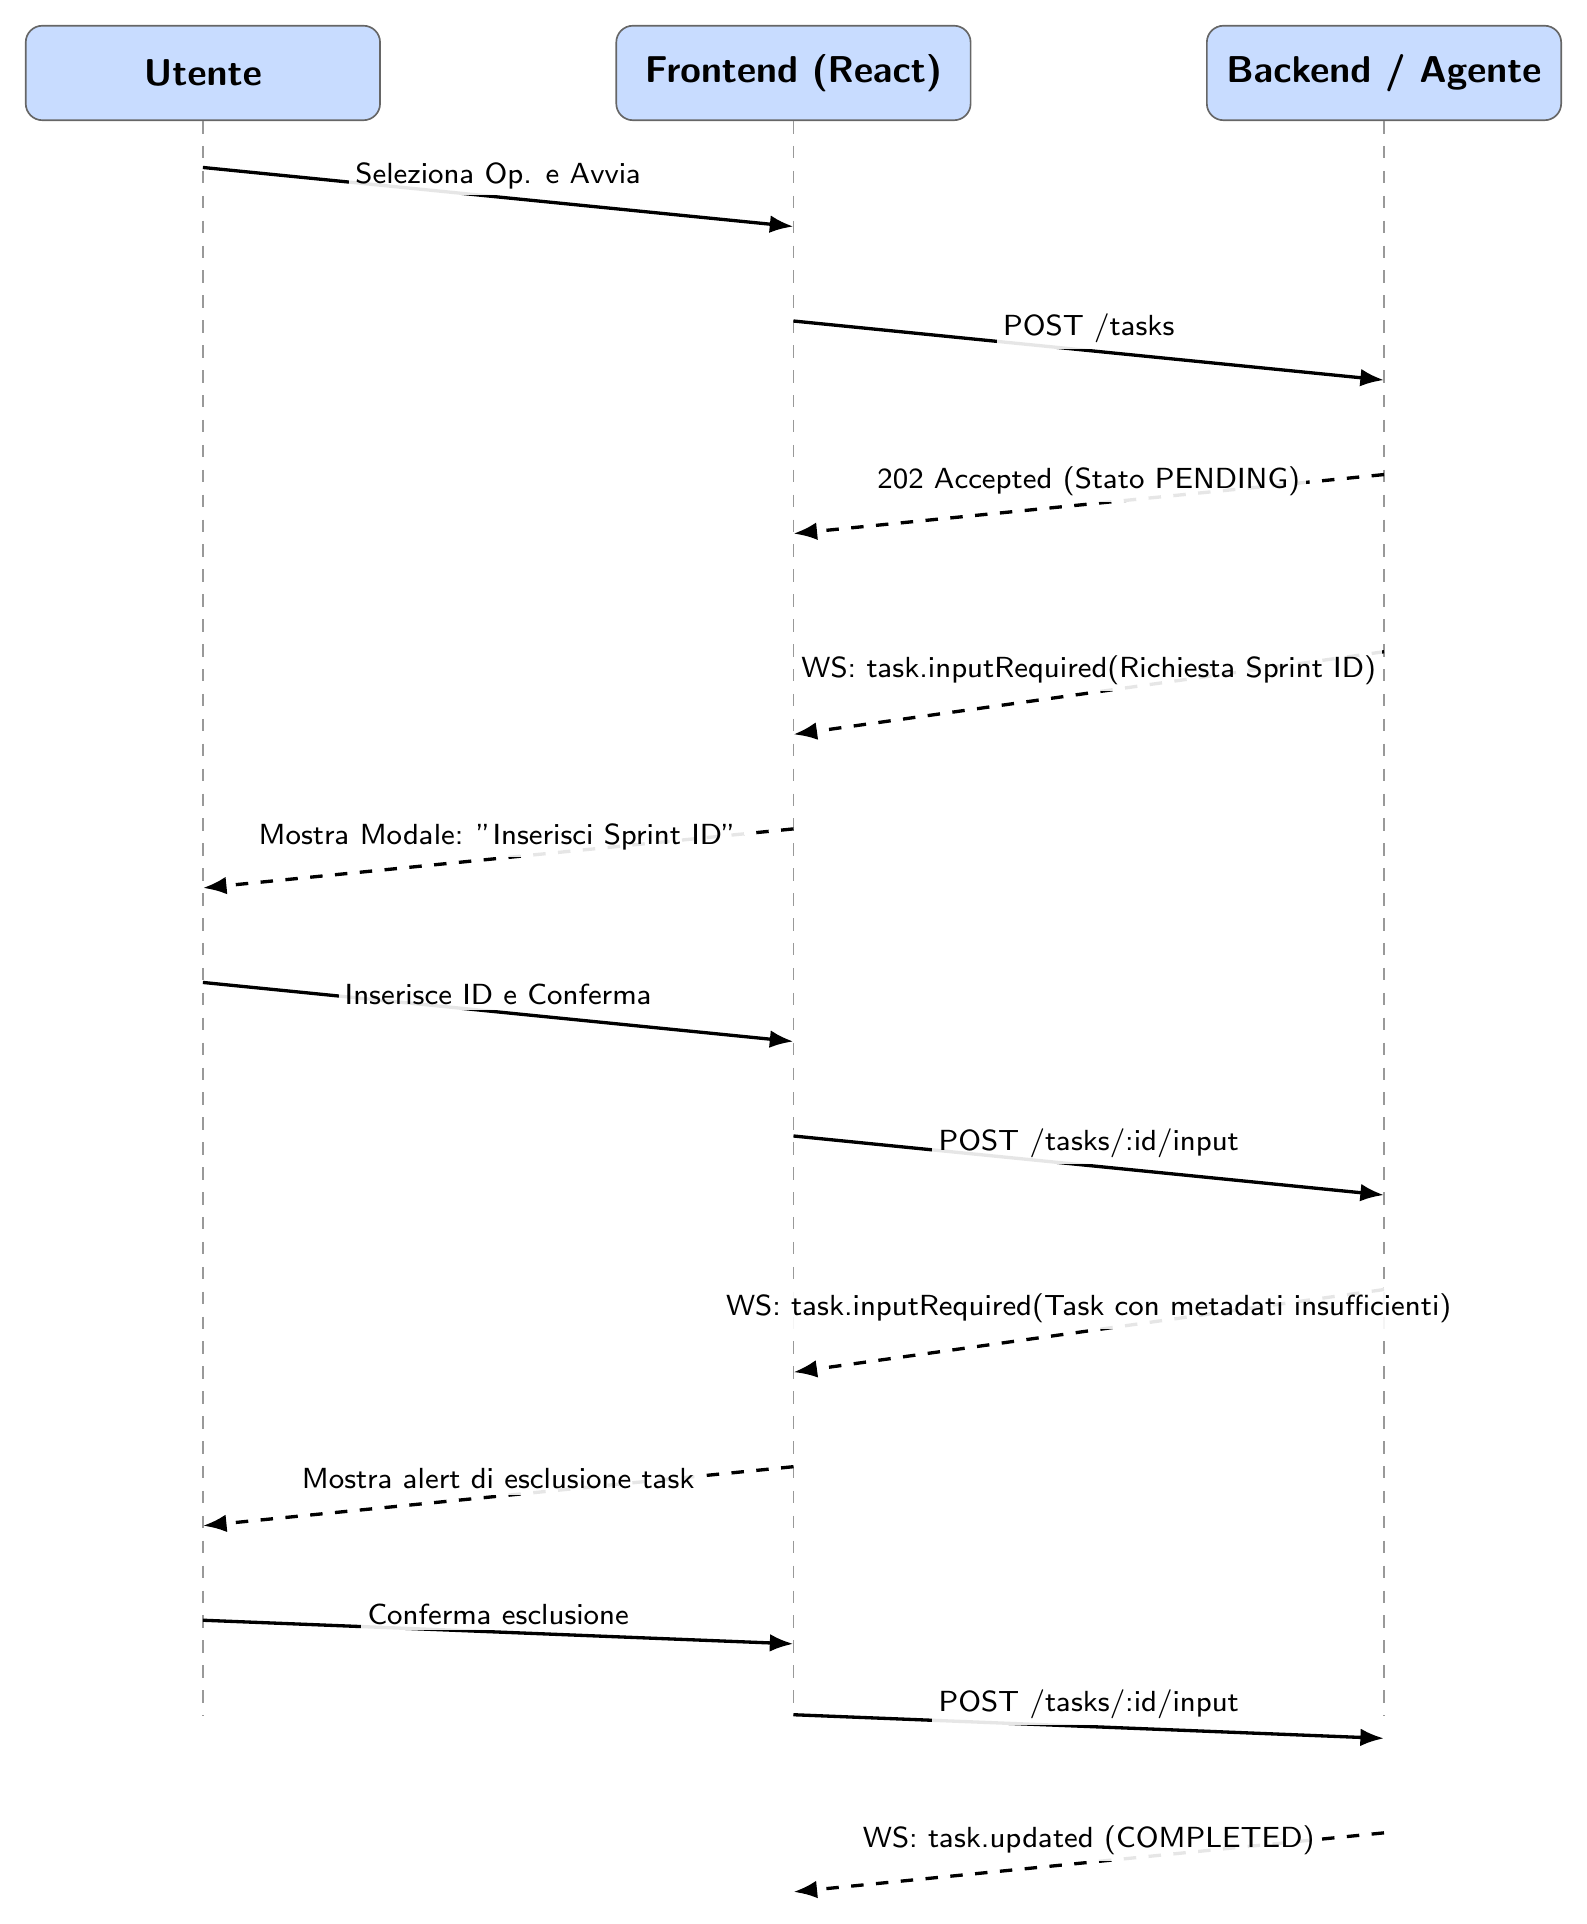
\includegraphics[width=0.85\textwidth]{figures/sequenza_changelog.png}
\caption{Sequenza di interazione tra utente e Agente Changelog durante l'elaborazione.}
\label{fig:changelog-seq}
\end{figure}

Come mostrato in Figura~\ref{fig:changelog-seq}, durante l'esecuzione possono comparire fino
a tre richieste, direttamente come area interattiva sull'elemento della Dashboard:

\begin{enumerate}
  \item \textbf{Richiesta dello Sprint ID} --- l'utente inserisce l'identificativo dello
        Sprint da cui estrarre le User Story completate, oppure annulla l'operazione;
  \item \textbf{Metadati insufficienti} --- se alcune User Story hanno una descrizione
        troppo povera per essere incluse in modo affidabile, l'utente sceglie se
        \textbf{procedere escludendole} oppure \textbf{annullare} l'intera operazione;
        vengono comunque riportate nel report come elenco delle esclusioni;
  \item \textbf{Conferma del changelog di business} --- solo per l'operazione di business:
        una volta generato il changelog tecnico intermedio, l'utente lo consulta in
        anteprima e sceglie se \textbf{accettare e generare il changelog di business}
        oppure \textbf{annullare}. Un rifiuto in questo passo annulla l'intera operazione:
        chi desidera solo il changelog tecnico può avviare direttamente quella singola
        operazione.
\end{enumerate}

Il changelog prodotto è un testo in formato Markdown, arricchito con i collegamenti
ipertestuali ai ticket di origine su GitHub. Il changelog di business viene inoltre
verificato dall'agente stesso per garantire un livello minimo di leggibilità prima di essere
restituito.

\subsection{Collegamento alla Pull Request}

Per tutte le operazioni dell'Agente Docs, il report include un collegamento diretto alla
Pull Request aperta automaticamente su GitHub al termine dell'elaborazione, insieme a
un'anteprima del diff proposto (consultabile ma secondaria rispetto al collegamento).
Nessun'altra azione è richiesta in Code Guardian: l'accettazione, il rifiuto o la richiesta
di modifiche avvengono normalmente su GitHub.

\subsection{Esportazione dei report in PDF}

Da qualunque pagina di dettaglio di un report è disponibile il pulsante \textbf{Esporta
PDF}, che genera e scarica un documento PDF con lo stesso contenuto mostrato a schermo. Il
file viene generato al momento della prima richiesta e riutilizzato per le richieste
successive, poiché il contenuto di un report non cambia nel tempo. Un eventuale fallimento
dell'esportazione non altera lo stato del report né il contenuto già visualizzato: viene
mostrato solo un messaggio d'errore temporaneo (si veda la sezione~\ref{sec:errori}).

% ============================================================
\newpage
\section{Risoluzione problemi ed errori}
\label{sec:errori}

\subsection{Due famiglie di errore}

Code Guardian distingue due tipi di errore, gestiti in modo diverso dall'interfaccia:

\begin{itemize}
  \item \textbf{Errori di validazione e configurazione} --- emergono immediatamente
        mentre si compila un modulo o si conferma una selezione (ad esempio un formato
        email non valido, un token GitHub mal formato). Il messaggio compare
        direttamente sotto il campo interessato e i dati già inseriti non vengono mai
        persi.
  \item \textbf{Errori di esecuzione} --- emergono a distanza di tempo dall'avvio di
        un'operazione, mentre l'agente sta lavorando, e vengono notificati in tempo reale.
        Solo l'operazione interessata passa allo stato \textbf{Fallito}: le altre
        proseguono senza interruzioni. Aprendo il report di un'operazione fallita, il
        contenuto normale viene sostituito da un riquadro che indica il tipo di errore,
        la fase in cui si è verificato e, quando disponibile, un'azione secondaria da
        intraprendere.
\end{itemize}

\subsection{Tabella degli errori più comuni}

La Tabella~\ref{tab:errori} elenca le cause più comuni di fallimento di un'operazione, il
messaggio che ci si può aspettare di vedere e l'azione consigliata.

\begin{longtable}{p{4.3cm}p{5.0cm}p{5.0cm}}
\toprule
\textbf{Causa} & \textbf{Messaggio tipico} & \textbf{Cosa fare} \\
\midrule
\endfirsthead
\toprule
\textbf{Causa} & \textbf{Messaggio tipico} & \textbf{Cosa fare} \\
\midrule
\endhead
Timeout del modello AI (\ecode{TIMEOUT}) &
Il modello AI ha impiegato troppo tempo a rispondere. &
\textbf{Riprova}: per rilanciare la sola operazione fallita. \\[4pt]
Output del modello non interpretabile (\ecode{PARSING}) &
L'output generato dall'AI non è nel formato atteso. &
\textbf{Riprova}: nella maggior parte dei casi un nuovo tentativo va a buon fine. \\[4pt]
Errore generico di sistema (\ecode{UPSTREAM}) &
Impossibile completare l'operazione per un errore interno di sistema. &
\textbf{Riprova}; se il problema persiste, contattare chi amministra l'applicazione. \\[4pt]
Ambito di analisi troppo esteso (\ecode{CONTEXT\_TOO\_LARGE}) &
Il contesto analizzato eccede la capacità di lettura del modello. &
Tornare a \route{/select} e ridurre l'ambito (selezionare meno file o cartelle). \\[4pt]
Risorsa mancante nel repository (\ecode{CONTEXT\_RESOURCE\_MISSING}) &
Risorsa richiesta non trovata (ad es. \texttt{POLICY.md} assente, Sprint ID inesistente). &
Verificare che la risorsa richiesta esista nel repository o nel Task Management, quindi
riavviare l'operazione. \\[4pt]
Risorsa non interpretabile (\ecode{CONTEXT\_RESOURCE\_INVALID}) &
La risorsa richiesta non è interpretabile. &
Controllare il formato della risorsa indicata (ad es. il file \texttt{POLICY.md}) e
correggerlo prima di riprovare. \\[4pt]
Limite di chiamate al modello AI (\ecode{LLM\_RATE\_LIMITED}) &
Limite di utilizzo del modello AI raggiunto; riprovare successivamente. &
Attendere qualche minuto prima di riavviare l'operazione. \\[4pt]
Leggibilità del changelog insufficiente (\ecode{READABILITY\_TOO\_LOW}) &
Il changelog di business generato non raggiunge la soglia minima di leggibilità richiesta. &
Rilanciare l'operazione; se il problema persiste, provare a ridurre l'ambito o lo Sprint
selezionato. \\[4pt]
Apertura Pull Request non riuscita (\ecode{PR\_CREATION\_FAILED}) &
Impossibile aprire la Pull Request; verificare i permessi del token. &
Controllare i permessi del token in \route{/credentials} e riavviare l'operazione. \\[4pt]
Limite mensile di operazioni raggiunto (\ecode{USAGE\_LIMIT\_EXCEEDED}) &
Limite di operazioni avviabili raggiunto per il periodo corrente. &
Attendere il rinnovo del periodo, oppure contattare chi amministra l'applicazione. \\[4pt]
Token GitHub scaduto o revocato (\ecode{CREDENTIAL\_INVALID}) &
Il token configurato non è più valido; verificalo su ``Servizi connessi''. &
Riconfigurare il token in \route{/credentials} (si veda la sezione~\ref{sec:credenziale-invalida}). \\
\bottomrule
\caption{Errori più comuni, messaggio mostrato e azione consigliata.}
\label{tab:errori}
\end{longtable}

\subsection{Credenziale GitHub non più valida}
\label{sec:credenziale-invalida}

Se durante l'esecuzione di un'operazione il token GitHub configurato risulta scaduto o
revocato, l'operazione in corso fallisce con l'errore \texttt{CREDENTIAL\_INVALID} e
l'applicazione mostra un banner persistente nell'intestazione, visibile su tutte le pagine,
finché la credenziale non viene sistemata. L'avvio di nuove operazioni resta bloccato nel
frattempo, mentre restano sempre consultabili le operazioni e i report già esistenti. Per
risolvere:

\begin{enumerate}
  \item aprire \route{/credentials} dal collegamento presente nel banner;
  \item generare un nuovo Personal Access Token su GitHub (o rinnovare i permessi di
        quello esistente);
  \item inserirlo nel campo del servizio GitHub e confermare: una volta validato, il
        banner scompare e l'applicazione torna pienamente utilizzabile.
\end{enumerate}

\subsection{Limite di utilizzo raggiunto}

Per contenere il consumo del modello AI, Code Guardian applica un limite al numero di
operazioni avviabili da ciascun utente in un mese solare. Se il limite viene raggiunto,
l'avvio di una nuova operazione (o di un intero lotto di operazioni avviate insieme) viene
rifiutato prima ancora che un agente venga interpellato: nessuna operazione del lotto
parte. Occorre attendere il rinnovo del periodo mensile oppure contattare chi amministra
l'applicazione per un eventuale innalzamento del limite.

\subsection{Altri casi frequenti}

\begin{itemize}
  \item \textbf{Il comando ``Esci'' mostra un errore} --- il logout richiede comunque una
        chiamata di rete; in caso di problemi di connessione può comparire un errore
        contestuale. La sessione locale, in ogni caso, viene comunque interrotta al
        successivo ricaricamento della pagina.
  \item \textbf{L'esportazione PDF fallisce} --- compare un messaggio temporaneo nella
        pagina del report, che resta comunque consultabile a schermo: è sufficiente
        premere di nuovo \textbf{Esporta PDF} per riprovare.
  \item \textbf{Il repository o il branch non vengono trovati} --- verificare che l'URL sia
        corretto e che il token configurato in \route{/credentials} abbia accesso al
        repository (per i repository privati, il token deve appartenere a un account con
        i permessi necessari).
\end{itemize}

% ============================================================
\newpage
\section{Glossario}

\begin{description}[leftmargin=3.4cm, style=nextline]
  \item[Agente] Componente basato su un modello linguistico (LLM) che esegue una specifica
    operazione di analisi o generazione (Docs, Security o Changelog) e restituisce un
    Report.
  \item[Ambito di analisi] La porzione del repository (intero contenuto, singoli file o
    cartelle) su cui un agente lavora, definita nella pagina \route{/select}.
  \item[Branch] Un ramo del repository Git; nella selezione del contesto rappresenta il
    riferimento di base su cui viene ancorata l'analisi.
  \item[Changelog di business] Sintesi delle novità di uno Sprint, scritta con un
    linguaggio accessibile a un pubblico non tecnico.
  \item[Changelog tecnico] Sintesi delle novità di uno Sprint orientata a un pubblico di
    sviluppatori, con collegamenti ai ticket di origine.
  \item[Commit] Un singolo salvataggio di modifiche nella cronologia del repository,
    identificato da un hash univoco; può essere usato come riferimento opzionale per
    ancorare un'analisi a un punto preciso della cronologia.
  \item[Contesto (di analisi)] L'insieme di repository, riferimento (branch/commit) e
    ambito selezionato, condiviso da tutte le operazioni avviate nella stessa sessione di
    lavoro.
  \item[Credenziale di servizio] Il Personal Access Token GitHub configurato dall'utente,
    che consente a Code Guardian di leggere codice e Issue per suo conto.
  \item[Dashboard] La pagina \route{/tasks}, che mostra in tempo reale lo stato delle
    operazioni avviate.
  \item[GitHub Issues] Il sistema di ticket di GitHub, usato in Code Guardian anche come
    sistema di gestione dei task/User Story letto dall'Agente Changelog.
  \item[JWT (token di sessione)] Il token che identifica una sessione utente autenticata;
    viene inviato automaticamente a ogni richiesta e non viene mai salvato in modo
    persistente nel browser.
  \item[LLM (Large Language Model)] Il modello linguistico di intelligenza artificiale su
    cui si basa ciascun agente per interpretare il codice e generare l'output.
  \item[OWASP Top 10] Elenco delle categorie di vulnerabilità di sicurezza più comuni nelle
    applicazioni web, usato come riferimento dalla Scansione vulnerabilità
    dell'Agente Security.
  \item[Personal Access Token (PAT)] Il token di accesso personale generato su GitHub,
    usato come credenziale di servizio.
  \item[POLICY.md] File presente nel repository che definisce le regole di sviluppo sicuro
    del progetto, verificato dall'operazione di conformità Policy-as-code.
  \item[Proposal] La modifica proposta da un agente sotto forma di diff (ad esempio un
    nuovo README), da cui viene generata automaticamente una Pull Request.
  \item[Pull Request (PR)] Una richiesta di modifica al repository, aperta automaticamente
    da Code Guardian al termine di un'operazione dell'Agente Docs; la sua revisione e
    approvazione avvengono su GitHub.
  \item[Repository] Archivio remoto, ospitato su GitHub, contenente il progetto software su cui vengono eseguite le
    analisi.
  \item[Report] Il risultato strutturato di un'operazione, consultabile nell'interfaccia
    ed esportabile in PDF.
  \item[Ruolo operativo] La specializzazione scelta in fase di registrazione (Sviluppatore,
    Security Auditor / Team Lead o Project Manager), che determina le operazioni
    disponibili.
  \item[Sprint] Un intervallo di lavoro del team, identificato da uno Sprint ID, da cui
    l'Agente Changelog estrae le User Story completate.
  \item[Task] Una singola operazione avviata (ad esempio una scansione di sicurezza),
    mostrata come elemento indipendente in Dashboard con un proprio stato e un proprio
    report.
  \item[WebSocket] Il canale di comunicazione in tempo reale tramite cui l'interfaccia
    riceve gli aggiornamenti di stato delle operazioni senza dover ricaricare la pagina.
\end{description}

\end{document}
